%% A simple template for a term report using the Hagenberg setup 
%% based on the standard LaTeX 'report' class

%%% Magic comments for setting the correct parameters in compatible IDEs
% !TeX encoding = utf8
% !TeX program = pdflatex 
% !TeX spellcheck = en_US
% !BIB program = biber

\RequirePackage[utf8]{inputenc} % Remove when using lualatex or xelatex!
\RequirePackage{hgbpdfa}        % Creates a PDF/A-2b compliant document

\documentclass[english,notitlepage,smartquotes]{hgbreport}
% Supported options in [..]:
%    Main language: 'german' (default), 'english'
%    Conversion to typographic quotation marks: 'smartquotes'
%    Use APA citation style: 'apa'
%    Do not create a separate title page: 'notitlepage'
%    Page layout: 'oneside' (single-sided, default), 'twoside' (double-sided)
%%%-----------------------------------------------------------------------------

\graphicspath{{images/}}  % Location of images and graphics
\bibliography{references} % Biblatex bibliography file (references.bib)
% theorems, definitions, remarks etc.
\usepackage{amsthm}

\theoremstyle{definition}
\newtheorem*{definition}{Definition}

\theoremstyle{remark}
\newtheorem*{remark}{Remark}

\theoremstyle{plain}
\newtheorem{theorem}{Theorem}[chapter]
\newtheorem{corollary}{Corollary}[theorem]
\newtheorem{lemma}{Lemma}[chapter]
\renewcommand\qedsymbol{$\blacksquare$}
% theorems, definitions, remarks etc.
% the "reflection" box
\usepackage[framemethod=tikz]{mdframed}
\newtheorem{reflection}{Reflection}
\mdfdefinestyle{reflectionbox}{
  linecolor=cyan,
  backgroundcolor=cyan!20,
}
\surroundwithmdframed[style=reflectionbox]{reflection}
% the "reflection" box

% long table
\usepackage{longtable}
% long table

% for algorithm description
\usepackage{algorithm}
\usepackage{algpseudocodex}
% for algorithm description
% for images etc.
\usepackage{tikz}
\newcommand*\circled[1]{\tikz[baseline=(char.base)]{
    \node[shape=circle,draw=red,inner sep=2pt] (char) {#1};}}
\newcommand*\fillcircled[2]{\tikz[baseline=(char.base)]{
    \node[shape=circle,fill=#2,draw=red,inner sep=2pt] (char) {#1};}}
% for images etc.
% color names
\usepackage[dvipsnames]{xcolor}
% color names
% Big starting letters
\usepackage{lettrine}
% Big starting letters
% cancel terms
\usepackage{cancel}
% cancel terms
% get rid of ugly borders
\hypersetup{
    colorlinks,
    linkcolor={magenta!50!black},
    citecolor={blue!50!black},
    urlcolor={blue!80!black}
}
% get rid of ugly borders

%%%-----------------------------------------------------------------------------
\begin{document}
%%%-----------------------------------------------------------------------------
\author{Kedar Mhaswade}                    % Your name
\title{Elementary Number Theory by Underwood Dudley:\\ % Name of the course or project
			Notes and Problem Solutions}	                 % or "Project Report"
\date{\today}

%%%-----------------------------------------------------------------------------
\maketitle
%%%-----------------------------------------------------------------------------
\begin{abstract}\noindent

\bigskip
\noindent
% Use the abstract to provide a short summary of the document's contents.
\lettrine[lines=3]{T}{his} is an objective, yet personal, narrative of the author's odyssey in the enchanted land of numbers. It contains his notes and solutions to problems from Professor Underwood Dudley's~\cite{Dudley2008} accessible introduction to Number Theory.

There is one issue with almost all books of rigorous mathematics (of the definition-theorem-lemma-proof style): they present mathematics in the \emph{finished} form\footnote{We assume that such a book is free from any egregious errors, typos etc.}. Proofs, however clear and lucid, are presented as if they are spoken by an omniscient Oracle. It's hard to imagine real humans doing mathematics this way from scratch. Countless hours need be spent on arriving at the presentable form. The author knew that and realized it again as he was writing his proofs\footnote{Almost all the proofs were first attempted with a pen on a lot of paper and then typeset. We live in an affluent society; the great mathematician Srinivasa Ramanujan didn't even have access to enough paper.}. He has attempted to point that out where possible. Running into dead ends and admitting it may disrupt the flow of normal reading (for reading mathematics is also like reading a careful disposition), but it may be reassuring especially to a beginning (but interested and, for the lack of a better word, intelligent) reader who is assumed author's companion. Delving too much into detours may ruin an otherwise readable travelogue. The author strives to seek a balance. \emph{Failed} proofs appear in this text with {\textcolor{red}{\Huge\bf ?}} instead of the QED symbol $\blacksquare$.

In the \emph{Preface} of his book Dudley writes,

``Number Theory problems can be difficult because inspiration is sometimes necessary to find a solution, and inspiration cannot be had to order. A student should not expect to be able to conquer all of the problems and should not feel discouraged if some are baffling. There is benefit in trying to solve problems whether a solution is found or not.''

We have all experienced the frustration and exaltation of solving problems. And, in arithmetic--the queen of mathematics--there is no dearth of beautiful and difficult problems. We should keep trying as long as doing so calmly feels worth the effort and brings joy. Destructive perfectionism is not needed. The author undertook this project almost purely as a labor of love\footnote{He also wanted to become a better programmer, but before he could solve the amazing \href{https://projecteuler.net/about}{\emph{Project Euler}} problems a bit more efficiently, he wanted to feel more comfortable with arithmetic!}. Doing mathematics (even established, not involving ``active mathematical research'') for the sake of it is sufficient because Professor Dudley has compellingly argued elsewhere (cf. \cite{DudCMJ1997}) that mathematics may not be necessary to find jobs, but it \emph{is} sufficient (to live a contented life).

Many a theorem (and lemma) in the book and its proof are provided. Attempt has been made to provide original (author's own) proofs (not verified by others). We mention it if a proof is reproduced verbatim from the book. Author's own proofs attempt to demonstrate an audacious, yet humble, renaissance attitude in the spirit of excellent collections like \cite{Pnftb2014} and \cite{Pftb2018}. Occasionally the author complements the beautifully austere nature of mathematics with modest emotional narratives (in the form of sidebars titled ``Reflection'').

A table of theorems (proved or researched) is compiled here [\ref{tab:theorems}]. We hope that the compilation proves valuable to readers. Readers interested only in problems and their solutions should look for the sections named ``Problems'' such as [\ref{sec:p1}]. Not all problems are equally exhilarating and solving every problem isn't exactly fun (See \cite{GarrettSO}).

Readable and flawless mathematical typesetting is hard. It's ironic that the epitome of exact sciences breeds a degree of inexactness in notation. Like in literature, meaning sometimes depends on context not captured in notation. And yet, an encyclopedic treatment of notation at the beginning of a work like this tends to bore readers\footnote{What disappointments them even more are typos and errors.}. Here too, a balance needs to be sought. A few conventions are therefore in order:
\begin{itemize}
\item A roman letter in italics, like, for example, $p$, denotes an integer, unless specified otherwise.
\item The so-called \verb|\cdot|: $\cdot$ to denote multiplication is sometimes omitted. Thus, $ab$ is equivalent (and often even preferred and ubiquitous, thanks to Euler!) to $a\cdot b$.

\end{itemize}
\end{abstract}

%%%-----------------------------------------------------------------------------
\tableofcontents
%%%-----------------------------------------------------------------------------

%%%-----------------------------------------------------------------------------
\chapter{Integers}
%%%-----------------------------------------------------------------------------

% Describe the initial goals and situation that lead to this project, requirements, as well as references to related work (\eg, \cite{Higham2020}).

\begin{definition}[Least-Integer Principle]
A nonempty finite set of integers contains a \emph{smallest element}.
\end{definition}
\begin{definition}[Divides]
\label{def:divides}
We say ``$a$ divides $b$'' and write $a\mid b$ if and only if there is an integer $d$ such that $ad=b$.

Thus, $a\mid b \iff \exists d\in \mathbb{Z} \text{\;such that\;} ad=b,  a, b\in \mathbb{N}$
\end{definition}

A few lemmas follow (straightforward proofs are omitted):
\begin{lemma}
\label{lemma:divides-sum}
If $d\mid a$ and $d\mid b$, then $d\mid(a+b)$.
\end{lemma}
\begin{lemma}
\label{lemma:divides-lin-comb}
If $d\mid a_1,d\mid a_2,\cdots, d\mid a_n$, then $d\mid(c_1a_1+c_2a_2+\cdots+c_na_n)$.
\end{lemma}
\begin{definition}[GCD]
\label{def:gcd}
We say $d$ is the ``greatest common divisor'' of $a$ and $b$ (not both zero) and write ``$d=\gcd(a, b)$'' if and only if
\begin{enumerate}
\item $d\mid a$ and $d\mid b$, and
\item $(c\mid a$ and $c\mid b)\implies c\leq d$
\end{enumerate}
\end{definition}

It follows that $\gcd(a, b)\geq 1$.

\begin{theorem}
\label{thm:gcd-multiple}
If $\gcd(a,b)=d$, then $\gcd(a/d, b/d)=1$.
\end{theorem}

\begin{proof}
We use proof by contradiction.

If $\gcd(a,b)=d$, then $\exists p,q\in\mathbb{Z}$ such that

\begin{equation}
\label{eq:a}
a=pd\implies a/d=p
\end{equation}
\begin{equation}
\label{eq:b}
b=qd\implies b/d=q
\end{equation}

From definition[\ref{def:gcd}], it follows that the $\gcd$ of any two natural numbers is greater than or equal to 1. 

Let us assume that $\gcd(p, q)=m>1$.

It then follows that $p=mx,q=my$ for some integers $x, y$.

From equations (\ref{eq:a}) and (\ref{eq:b}), we get:
$$
a=mxd
$$
and
$$
b=myd
$$

Then, $\gcd(a, b)=md$. Since $m>1$, $\gcd(a, b) > d$.

This is a contradiction because we had $\gcd(a,b)=d$. Therefore, our assumption $\gcd(p,q)=m>1$ is incorrect and we must have $\gcd(p,q)=\gcd(a/d,b/d)=1$.
\end{proof}
\begin{definition}[Relatively Prime]
We say that $a$ and $b$ are \emph{relatively prime} if and only if $\gcd(a,b)=1$.
\end{definition}

\begin{theorem}
\label{thm:div-algo}
Given positive integers $a$ and $b$, there exist two unique integers $q$ and $r, 0\leq r<b$ such that  
$$
a=bq+r
$$
\end{theorem}
\begin{proof}
We first prove the existence of integers, $q,r$ by cases. For positive integers $a$ and $b$ there are three possibilities:
\begin{enumerate}
\item $a < b$

Since $a=b\cdot 0+a$, we get $q=0$ and $r=a$ as the two integers. 
\item $a=b$

Since $a=b=b\cdot 1+0$, we get $q=1$ and $r=0$ as the two integers. 
\item $a > b$

This means that $b$ can be subtracted $q\geq 1$ times from $a$ for the result of the subtraction ($a-q\cdot b$) to remain non negative. The result would be negative if we subtracted $b$ once more (that is, $q+1$ times in all) from $a$. The result of the subtraction, $a-q\cdot b$, which we denote as $r$, must then be a positive integer less than $b$, because otherwise we could subtract $b$ at least once more.
\end{enumerate}

We have proved the existence of the two integers $q$ and $r$ and demonstrated how to find them in all the cases. 

The above proof of existence describes a precise, deterministic procedure to find non negative integers $q$ and $r$ for any positive integers $a$ and $b$. However, we need to prove that the pair is unique. We prove uniqueness by contradiction.

Let $q_1\ne q$ and $r_1\ne r$ be \emph{another pair of non negative integers} produced by the procedure above. We have
\begin{equation}
\label{eq:qr}
a=bq+r
\end{equation}
and
\begin{equation}
\label{eq:q1r1}
a=bq_1+r_1
\end{equation}

From the existence proof above, $r<b$ and $r_1<b$.

It follows from equations (\ref{eq:q1r1}) and (\ref{eq:qr}) that
$$
b\cdot(q-q_1)=r_1-r
$$

From the definition (\ref{def:divides}) it then follows that $b\mid(r_1-r)$. However, $r_1<b\implies r_1-r<b-r\implies r_1-r<b$. This is a contradiction unless $r_1-r=0$, or $r_1=r$. If $r_1=r$, $q_1=q$ proving uniqueness.
\end{proof}

We call $q$ the \emph{quotient} and $r$ the \emph{remainder}. Theorem [\ref{thm:div-algo}] is called an ``algorithm'' because it entails a precise procedure to calculate non negative integers $q$ and $r$ for integers $a$ and $b$ (not both zero). The book correctly mentions that the theorem also holds when either $a$ or $b$ (or both) are negative. However, when negative numbers are involved, additional care must be exercised.

Consider, for example, $a=5$ and $b=-2$. Then, $a=b\cdot (-3)+(-1)$ giving $q=-3$ and $r=-1$. Moreover, $a=b\cdot (-2)+1$ giving $q=-2$ and $r=1$. Doesn't the uniqueness of division algorithm hold? For $0\leq r$ we must reject $r=-1$, whereas for $r<b$ we must reject both $r=1$ and $r=-1$. If we change the constraint on $r$ to $0\leq r<-b$ however, we allow the second case and achieve uniqueness. 

The division algorithm is most commonly applied to non negative integers.
\begin{lemma}
\label{lemma:gcd-pre}
If $a=bq+r$ where $0\leq r<b$, then $\gcd(a,b)=\gcd(b,r)$
\end{lemma}
\begin{proof}
We give a straightforward deductive proof.

Consider a common divisor (not necessarily the greatest) $c$ of $a$ and $b$. Then, by definition,

$$
a=c\cdot m_1
$$
$$
b=c\cdot m_2
$$

Then, $a=b\cdot q+r\implies c\cdot m_1=c\cdot m_2\cdot q+r$.

$\therefore r=c\cdot(m_1-q\cdot m_2)\implies c\mid r$

This means $c$ is a divisor of $r$. The reasoning applies to all common divisors of $a$ and $b$, and, therefore, it also applies to the greatest of them all--the $\gcd(a,b)=g_{ab}$. 

We proved that $g_{ab}$ is a divisor of $r$. We still need to prove that $g_{ab}$ equals $\gcd(b,r)=g_{br}$. 

Let us use contradiction to prove that. Let us \emph{assume} $g_{br}>g_{ab}$. This implies that $g_{br}$ divides $b$ and $r$ but does \emph{not} divide $a$. 

However, $a=bq+r\implies \exists x,y\in\mathbb{N}\mid a=(g_{br}\cdot x)q+g_{br}\cdot y$

$\therefore a=g_{br}(qx+y)\implies g_{br}\mid a$---a contradiction owing to our faulty assumption that $g_{br}>g_{ab}$ does not divide $a$.

There is no such $g_{br}>g_{ab}$. Therefore, $\gcd(a,b)=\gcd(b,r)$.
\end{proof}

\begin{reflection}
This--a divisor of $a$ and $b$ must be a divisor of $r$-- is one of Euclid's remarkable observations. The author never solemnly paused in its admiration in grade school. Perhaps that was because loving numbers for the sake of it did not cross his mind then.

The author's obsession for numbers is still rudimentary, but the above proof that he wrote down using a paper and a pen on an airplane gave him ineffable joy; he understood Euclid's argument better and, in that moment, like Piaget \cite{Piaget1974} observed, he \emph{momentarily became Euclid}! 
\end{reflection}

Greeks showed signs of computational excellence when finding $\gcd(a,b)$. They used the above lemma [\ref{lemma:gcd-pre}] to confidently reduce the size of the problem: to find the $\gcd$ of two numbers($a\geq b$ and $b$), find the remainder $r$ by applying the division algorithm to $a,b$ and find the $\gcd$ of two smaller numbers ($b>r$ and $r$)\footnote{$\gcd(a,b)$ also equals $\gcd(a,r)$, but their choice--$\gcd(b,r)$--was perhaps computationally more efficient}! They, unlike we did in grade school, never listed all the divisors of both the numbers and chose the largest of the common ones.

We define the `remainder operation' on two integers $a$ and $b$ (denoted `$a\mod b$') to return the remainder by applying the division algorithm [\ref{thm:div-algo}] to $a$ and $b$.

Dudley gives an \emph{iterative} procedure for Euclid's $\gcd$ algorithm next. However, we give an arguably more expressive recursive algorithm that uses a corollary that the $\gcd$ of a non negative number $a$ and $0$ is $a$. 

\begin{algorithm}
\begin{algorithmic}
\caption{Euclid's $\gcd(a,b)$ Algorithm}
\label{alg:euclid}
  \If{$b=0$}
    \State return a
  \Else
    \State return $\gcd(b,a\mod b)$
  \EndIf
\end{algorithmic}
\end{algorithm}

This can also be expressed inductively using \emph{cases}:
\[
\gcd(a,b)=
\begin{cases}
a& \text{if $b=0$}, \\
\gcd(b,a\mod b)& \text{otherwise}
\end{cases}
\]

We provide proofs of \emph{correctness} of algorithms. For Algorithm [\ref{alg:euclid}], if $b=0$, the algorithm immediately terminates producing the correct result ($a$). If $b\ne 0$, then division algorithm applies and we find the $\gcd$ of $b$ and a number less than $b$ (because the remainder, $r$, is such that $0\leq r<b$). The process continues till the second argument becomes $0$. Since $b$ is finite and the second argument is guaranteed to reduce by at least $1$ every time the division algorithm applies. Such reduction must stop when the remainder becomes $0$ and the algorithm terminates and returns the first argument, $a$, the $\gcd$ of the original numbers. 

\begin{reflection}
A few thoughts occurred to the author:
\begin{enumerate}
\item Is a \emph{descent} through Euclid's $\gcd$ algorithm like $(a,b)\rightarrow(b,b-1)\rightarrow(b-1,b-2)\dots\rightarrow(1,0)$ possible? When does the algorithm perform the best and worst?
\item Are any two consecutive Fibonacci numbers relatively prime? Does an invocation of $\gcd(F_{n+1}, F_n)$ \underline{always} result in finding $gcd$ of the lower Fibonacci numbers\footnote{\emph{Preliminary} tests seem to suggest so\dots}.
\end{enumerate}
\end{reflection}

\begin{theorem}
\label{thm:bezout-idty}
If $\gcd(a,b)=d$, then $\exists x,y\in\mathbb{Z}\mid ax+by=d$.

(Informally: $\gcd(a,b)$ can be expressed as a linear combination of $a$ and $b$ with integer coefficients.)
\end{theorem}
\begin{proof}\renewcommand{\qedsymbol}{\textcolor{red}{\Huge\bf ?}}
We give an algebraic proof.

$$
d=\gcd(a,b)\implies d\mid a\implies a=m_1\cdot d; m_1\in\mathbb{N}
$$
$$
d=\gcd(a,b)\implies d\mid b\implies b=m_2\cdot d; m_2\in\mathbb{N}
$$

It follows that
$$
a\cdot m_2=b\cdot m_1
$$
$$
\therefore a\cdot m_2+d=b\cdot m_1+d
$$
$$
\therefore a\cdot (m_2-1)+a+d=b\cdot m_1+d
$$
$$
\therefore a\cdot (m_2-1)+m_1\cdot d+d=b\cdot m_1+d
$$
\end{proof}
\begin{reflection}
The author intended to achieve a proof through a simple algebraic manipulation that was not to be! His intention was to determine a deterministic procedure to express $gcd(a, b)$ as a linear combination $ax+by$ of the integers $a$ and $b$. But he realized that such a manipulation was not as straightforward as he initially imangined. 

He also realized that the theorem holds only for the $\gcd$ and not for any other common divisor. For example, for $42$ and $18$, whose $\gcd$ is 6, the theorem states that $\exists x, y$, $42x+18y=6$; this couldn't be extended to another common divisor of $42$ and $18$ like $1$ or $3$ because we immediately run into a contradiction like $42x+18y=1$ or $42x+18y=3$ (the left hand side is an even number and the right hand side is an odd number).

Therefore, $\gcd(a,b)$ represents something more about $a$ and $b$ than what their other common divisors do.
\end{reflection}

To prove [\ref{thm:bezout-idty}], Dudley hints at \emph{working backwards} from the descent of numbers $a$ and $b$ in a continued application of the division algorithm [\ref{thm:div-algo}] as long as $b$ remains nonzero. We attempt that below.

But first, let's consider an example: Find the $\gcd$ of $a=222$ and $b=60$.

\begin{align*}
222&=\circled{60}\times3+\circled{42}\\
60&=\circled{42}\times1+\circled{18}\\
42&=\circled{18}\times2+\circled{6}\\
18&=\circled{6}\times3+\circled{0}
\end{align*}

$\therefore\gcd(222,60)=6$.\\

Working backwards through the descent (and eliminating 42 and 18 in the process) we get:
\begin{align*}
6&=42-\circled{18}\times 2\\
6&=42-(60-42\times 1)\times 2=\circled{42}\times 3-60\times 2\\
6&=(222-60\times 3)\times 3-60\times 2=222\times 3-60\times 11\\
6&=222\cdot 3+60\cdot(-11)\\
\\
\therefore x=3,y=-11
\end{align*}



\begin{proof}
Let's apply the division algorithm [\ref{thm:div-algo}] continuously, starting with $a$ and $b$. We know from above that this descent must eventually result in the application of the division algorithm to some integer and 0 yielding the $\gcd(a,b)$.

Let $r_n=0$, then $r_{n-1}=d=\gcd(a,b)$.

\begin{align*}
a&=bq_1+r_1\\
b&=r_1q_2+r_2\\
r_1&=r_2q_3+r_3\\
r_2&=r_3q_4+r_4\\
&\;\;\vdots \notag \\
r_{n-4}&=r_{n-3}q_{n-2}+r_{n-2}\\
r_{n-3}&=r_{n-2}q_{n-1}+d\\
r_{n-2}&=dq_n\;(r_n=0)
\end{align*}

We start with an expression for the $\gcd$ and work backwards to eliminate one number (from the step above) at a time. Every eliminated number yields a linear combination of remaining two numbers. This process evetually stops when $a$ and $b$ remain. Since every expression is a linear combination of integers starting with $r_{n-3}$ and $r_{n-2}$ which get eliminated in steps.

\colorbox{BurntOrange}{Need to make the proof tighter.}
\end{proof}

Theorem [\ref{thm:bezout-idty}] that $\exists x,y\in\mathbb{N}\mid ax+by=\gcd(a,b)$ is called B\'ezout's Identity. 

Are $x$ and $y$ thus found unique for the given $a$ and $b$?\\

No. For example, for $a=42$ and $b=18$:
\begin{align*}
42\times 1+18\times(-2)&=6\implies(x,y)=(1,-2)\\
42\times(-2)+18\times(5)&=6\implies(x,y)=(-2,5)\\
42\times 4+18\times(-9)&=6\implies(x,y)=(4,-9)\\
\vdots
\end{align*}


Is this (working backwards through the descent) the only way to find $x$ and $y$ for the given $a$ and $b$?

Dudley asserts that we can devise another method to determine $x$ and $y$. Let's see.

The equation $ax+by=d\mid a,b,x,y\in\mathbb{Z}$ is the so-called \emph{Linear Diophantine Equation} \cite{Dio} and is a special case of the general Diophantine equation. Solving such equations for (integer) solutions for given $a,b$ has a rich history. See \cite{MartinHershSciAm} for an accessible and fascinating introduction.

We have three corollaries from B\'ezout's Identity.
\begin{corollary}
\label{cor:ddivab}
If $d\mid ab$ and $\gcd(d,a)=1$, then $d\mid b$.

(Informally: If an integer $d$ divides the product of two integers $a$ and $b$ and if $d$ and one of $a$ and $b$ are relatively prime, then the other must be a multiple of $d$.)
\end{corollary}
\begin{proof}
We give a straightforward proof\footnote{Of course, other proofs, for example, one based on prime factorization of integers, are possible.} based on B\'ezout's Identity (Theorem ~\ref{thm:bezout-idty}).

B\'ezout's Identity when applied to the fact that $d$ and $a$ are relatively prime (i.e. $\gcd(d,a)=1$) gives us
$$
\exists x,y\in\mathbb{Z}\mid dx+ay=1
$$
$$
\therefore d\cdot b\cdot x+a\cdot b\cdot y=b
$$
But, $d\mid a\cdot b\implies a\cdot b=m_1\cdot d$, $m_1\in\mathbb{N}$
$$
\therefore d\cdot b\cdot x+m_1\cdot d\cdot y=b
$$
and
$$
d\cdot(bx+m_1y)=b
$$
This means $d\mid b$ because $bx+m_1y$ is an integer since the set of integers is closed under addition and multiplication.
\end{proof}

It's crucial that $d$ and $a$ are relatively prime for the corollary [\ref{cor:ddivab}] to hold.
\begin{corollary}
\label{cor:cdivd}
Let $\gcd(a,b)=d$, and suppose $c\mid a$ and $c\mid b$. Then $c\mid d$.

(Informally: A common divisor of two integers is a divisor of their $\gcd$.)
\end{corollary}
\begin{proof}
We give a rather straightforward proof based on B\'ezout's Identity (Theorem \ref{thm:bezout-idty}).
\begin{equation}
\label{eq:cdivd}
\exists x,y\in\mathbb{Z}\mid ax+by=d
\end{equation}
Also,
$$
c\mid a\implies \exists m_1\in\mathbb{N}\mid a=m_1\cdot c
$$
and
$$
c\mid b\implies \exists m_2\in\mathbb{N}\mid b=m_2\cdot c
$$
Then, it follows from equation (\ref{eq:cdivd}) that
$$
m_1cx+m_2cy=d
$$
and
$$
c(m_1x+m_2y)=d\implies c\mid d
$$

\end{proof}
\begin{corollary}
\label{cor:abdivm}
If $a\mid m$, $b\mid m$, and $\gcd(a,b)=1$, then $ab\mid m$.

(Informally: The product of two relatively prime divisors of an integer is its divisor.)
\end{corollary}
\begin{proof}
Once again we give a straightforward proof based on B\'ezout's Identity (Theorem \ref{thm:bezout-idty}).
We have
$$
a\mid m\implies m=c_1\cdot a,
$$
$$
b\mid m\implies m=c_2\cdot b,
$$
\begin{equation}
\label{eq:msq}
\therefore m^2=c_1c_2ab,
\end{equation}
and
$$
\gcd(a,b)=1\implies \exists x,y\in\mathbb{Z}\mid ax+by=1
$$
$$
\therefore axc_1c_2+byc_1c_2=c_1c_2
$$
From which, it follows that
\begin{equation}
\label{eq:mk}
mxc_2+myc_1=c_1c_2\implies mk=c_1c_2 \;\;\;(\because xc_2+yc_1=k)
\end{equation}
From equations (\ref{eq:msq}) and (\ref{eq:mk})
$$
m^2=mkab\implies m=kab\implies ab\mid m
$$
\end{proof}
\section*{Problems}
\label{sec:p1}
We solve a number of problems below.
\begin{enumerate}[label=\textbf{\arabic*}.]
\item Calculate $\gcd(314,159),\gcd(4144,7696)$
\label{pr:11}

We apply Euclid's $\gcd$ Algorithm (\ref{alg:euclid}).

\begin{align*}
314&=\circled{159}\times 1+\circled{155}\\
159&=\circled{155}\times 1+\circled{4}\\
155&=\circled{4}\times 38+\circled{3}\\
4&=\circled{3}\times 1+\circled{1}\\
3&=\fillcircled{1}{cyan!20}\times 3+\circled{0}
\end{align*}
$\therefore \gcd(314,159)=1$.

\begin{align*}
4144&=\circled{7696}\times 0+\circled{4144}\\
7696&=\circled{4144}\times 1+\circled{3552}\\
4144&=\circled{3552}\times 1+\circled{592}\\
3552&=\fillcircled{592}{cyan!20}\times 6+\circled{0}\\
\end{align*}

$\therefore \gcd(4144,7696)=592$.

\item Calculate $\gcd(3141,1592),\gcd(10001,100083)$
\label{pr:12}

Although nothing is exactly useless, some things can be boring and so we omit some details!
\begin{align*}
3141&=\circled{1592}\times 1+\circled{1549}\\
1592&=\circled{1549}\times 1+\circled{43}\\
\vdots
\end{align*}

$\therefore \gcd(3141,1592)=1$ and $\gcd(10001,100083)=73$.

\item Find $x,y\in\mathbb{Z}\mid 314x+159y=1$.\\
\label{pr:13}

We have established that $\gcd(314,159)=1$ above (\ref{pr:11}), without which there would be no integral $x,y$ that satisfy this linear Diophantine equation.

One way to get the desired solution is to work backwards through the descent:

\begin{align*}
4&=(155-4\times 38)\times 1+\fillcircled{1}{cyan!20}\\
4\times 39-155\times 1&=\fillcircled{1}{cyan!20}\\
(159-155)\times 39-155\times 1&=\fillcircled{1}{cyan!20}\\
159\times 39-155\times 40&=\fillcircled{1}{cyan!20}\\
159\times 39-(314-159)\times 40&=\fillcircled{1}{cyan!20}\\
314\times(-40)+159\times(79)&=\fillcircled{1}{cyan!20}
\end{align*}

$\therefore x=-40,y=79$ is a solution to the linear Diophantine equation $314x+159y=1$.

\item Find $x,y\in\mathbb{Z}\mid 4144x+7696y=592$.\\
\label{pr:14}

This `problem' is left as an exercise to readers.

\item If $N=abc+1$, prove that $\gcd(N,a)=\gcd(N,b)=\gcd(N,c)=1$. 
\label{pr:15}
\begin{proof}
We use the division algorithm [\ref{thm:div-algo}].
$$
\because N=a(bc)+1 \therefore \gcd(N,a)=\gcd(a,1)
$$
And since $1\mid x\forall x\in\mathbb{Z}, \gcd(x,1)=1$.

$\therefore 1=\gcd(a,1)=\gcd(N,a)$.

Similar argument can be used to prove relative-primality of $N,b$ and $N,c$. 
\end{proof}

\item Find \emph{two different\footnote{Perhaps for emphasis; ``two'' implies ``two different''.}} solutions of $299x+247y=13$.
\label{pr:16}

Let's first establish that at least one (integral) solution exists. Because of [\ref{thm:bezout-idty}], our job is easier:

\begin{align*}
299&=\circled{247}\times 1+\circled{52}\\
247&=\circled{52}\times 4+\circled{39}\\
52&=\circled{39}\times 1+\circled{13}\\
39&=\fillcircled{13}{cyan!20}\times 3+0
\end{align*}
$\because\gcd(299,247)=13 \therefore \exists x,y\in\mathbb{Z}\mid 299x+247y=13$.

Working backwards through a familiar descent we get: $x=5,y=-6$ as one solution.
\begin{reflection}
Interestingly, Dudley asks for two solutions! In a way, he's nudging us to be creative! He has said somewhere that we'll learn about finding different solutions to the linear Diophantine equation given by B\'ezout's Identity. However, we can try on our own.

Are other corollaries or lemmas likely to help us?

Does another solution exist? How many solutions are there?

These are all hard questions. They express the difficulty of doing mathematics and of developing an \underline{inductive} thinking, however limited in influence. For example, if we are unfamiliar with the ``theory of linear Diophantine equations'' what makes us take a \underline{leap of faith}\footnote{The author borrows this term from a lucid book, \emph{Thinking Recursively}, by Eric Roberts \cite{Roberts1986}, which introduces a `recursive leap of faith'.} that another solution exists?

We believe that try sensibly we must. We may be in dark. However, unless we, guided by established knowledge and fueled by imagination, explore the mysterious, how might we uncover new knowledge(even at a personal level)? A ``solved problem'' is unsolved for us until we solve it (first somehow, then by application of an established theory or technique).
\end{reflection}

$$
297x+247y=13\implies 13(23x+19y)=13\implies 23x+19y=1
$$

The above implies that \emph{every} solution of $23x+19y=1$ is a solution of $297x+247y=13$ and vice versa. Therefore, $(x,y)=(5,-6)$ is a solution\footnote{The familiar ascent through the repeated application of the division algorithm yields the same solution.} of $23x+19y=1$.

Does $23x+19y=1$ have \emph{another} solution?

It's easier to try with smaller numbers. Any generalization starts with some concrete experiments. Consider an experiment tabularized below:

\begin{table}[h!]
\centering
\begin{tabular}{|c|c|c|c|}
 \hline
 $x$ & $y$ & $23x+19y$ &Multiples of $(23-19)$ that yields $1$ from $23x+19y$\\ [0.5ex]
 \hline
 1 & $-1$ & 4 &--\\\hline
 1 & $-2$ & \fillcircled{-15}{cyan!20} &$4,\fillcircled{-15}{cyan!20}+(23-19)\times 4=1$\\\hline
 1 & $-3$ & -34 &--\\\hline
 1 & $-4$ & -53 &--\\\hline
 1 & $-5$ & -72 &--\\\hline
 1 & $-6$ & \fillcircled{-91}{cyan!20} &$23,\fillcircled{-91}{cyan!20}+(23-19)\times 23=1$\\\hline
 \vdots & \vdots & \vdots&\vdots\\\hline
 1 & $-10$ & \fillcircled{-167}{cyan!20} &$42,\fillcircled{-167}{cyan!20}+(23-19)\times 42=1$\\\hline
\end{tabular}
\caption{How $23x+19y$ Changes}
\label{tab:23x19y}
\end{table}

Consider the first row in the Table \ref{tab:23x19y}. We observe that since $23(1)+19(-2)=-15$, $23(1)+19(-2)+(23-19)4=23(5)+19(-6)$ yields 1. Only if $23x+19y=4k-1,k\in\mathbb{Z}$, then we can expect $23x+19y+k(23-19)=23(k-x)+19(y-k)$ to yield $1$.

That---$x=5$ and $y=-6$---was our first solution. Values of $x$ and $y$ for which $23x+19y\ne4k-1$ are not of our interest. Now consider $x=1$ and $y=-6$. Since $23(1)+19(-6)=-91$, $23(1)+19(-6)+(23-19)23=23(24)+19(-29)$ also yields 1. Therefore, $x=24$ and $y=-29$ is another solution. Yet another is $x=43$ and $y=-52$.

Perhaps there is some arithmetic progression lurking here, because the next solution ($62,-75$) will be given by the row for $x=1, y=-14$. 

This process can continue. Infinitely many solutions starting with $(5,-6)$ are possible. If $(p, q)$ is a solution, then $(p+19k,q-23k)$ is also a solution of the linear Diophantine equations $23x+19y=1$ and $299x+247y=13$:
\begin{align*}
&(5,-6)\\
&(24,-29)\\
&(43,-52)\\
&(62,-75)\\
\vdots
\end{align*}
\begin{reflection}
Did we get lucky there?

Perhaps we did.

We cannot escape a feeling that we are close to a useful generalization, a slice of a theory! We will carry that positive feeling along but curb our enthusiasm.
\end{reflection}
\item Prove that if $a\mid b$ and $b\mid a$, then $a=b$ or $a=-b$.
\label{pr:17}
\begin{proof}
We give a straightforward proof.
$$
a\mid b\implies \exists c\in\mathbb{Z}\mid b=ca 
$$
and
$$
b\mid a\implies \exists d\in\mathbb{Z}\mid a=db 
$$
It follows that
$$
ab=cdab
$$
If $a\ne0,b\ne0$, then 
$$
cd=1
$$
This is possible only if $c=1,d=1$ or $c=-1,d=-1$. It then follows that either $a=b$ or $b=-a$ i.e. $a=-b$.
\end{proof}

\item Prove that if $a\mid b$ and $a>0$, then $\gcd(a,b)=a$.
\label{pr:18}
TBD

\item Prove that $\gcd(\gcd(a,b),b)=\gcd(a,b)$.
\label{pr:19}
\begin{proof}
Here's a straightforward proof.

Consider all the \emph{common} divisors of $a$ and $b$ listed in an ascending order: 
$$
d_1>d_2>\dots>d_n
$$

Then, by definition, $d_1=1$ and $d_n=\gcd(a,b)$.

Again, by definition, $d_n\mid b$ and, trivially, $d_n\mid d_n$. Therefore, $d_n=\gcd(a,b)$ divides $b$ and $\gcd(a,b)$. There is no greater common divisor. Therefore, $\gcd(\gcd(a,b),b)=\gcd(a,b)$.

\end{proof}
\item
\begin{enumerate}
\item Prove that $\gcd(n,n+1)=1\forall n>0$.
\label{pr:110a}
\begin{proof}
$\because\gcd(0,a),a>0=a,\therefore\gcd(0,1)=1$.

We argue based on the fact $\text{for } a,b\in\mathbb{Z}, ab=1\implies a=1,b=1, \text{or } a=-1,b=-1$.

Let $\gcd(n,n+1)=d$.

Then, $\exists p,q\in\mathbb{Z}$ such that
$$
n=pd
$$
$$
n+1=qd
$$
It follows that
$$
(q-p)d=1
$$
Therefore (also since $q-p\in\mathbb{Z}$), either
$$
(q-p)=1,d=1
$$
, or
$$
(q-p)=-1,d=-1
$$
$$
\because d>0, \therefore d=1,q-p=1
$$

$\therefore \gcd(n,n+1)=1\forall n\geq 0$.

\end{proof}
\begin{proof}
\label{proof:nn+1}
We give an alternative proof using the division algorithm\footnote{It occurred to the author at a hospital waiting room.}.

$$
\gcd(n,n+1)=\gcd(n+1,n)
$$

But $n+1=\circled{$n$}\cdot 1 + \circled{$1$}$.
$$
\therefore \gcd(n+1,n)=\gcd(n,1)=1
$$

\end{proof}
\item If $n>0$, what can $\gcd(n,n+2)$ be?

\label{pr:110b}
It has got to be either 0 or 1.
\begin{proof}
We argue as in the above (alternative) proof (\ref{proof:nn+1}).

\begin{align*}
n&=\circled{$n+2$}\cdot 0+\circled{$n$}\\
n+2&=\circled{$n$}\cdot 1+\circled{2}
\end{align*}

$\therefore\gcd(n,n+2)=\gcd(n,2)$.

\[
\gcd(n,2)=
\begin{cases}
1& \text{if $n$ is odd}, \\
2& \text{otherwise}
\end{cases}
\]

\end{proof}
\end{enumerate}
\item 
\begin{enumerate}
\item Prove that $\gcd(k,n+k)=1$ if and only if $\gcd(k,n)=1$.

TBD

\item Is it true that $\gcd(k,n+k)=d$ if and only if $\gcd(k,n)=d$?

TBD
\end{enumerate}

\item Prove: If $a\mid b$ and $c\mid d$, then $ac\mid bd$.

TBD

\item Prove: If $d\mid a$ and $d\mid b$, then $d^2\mid ab$.

This `problem' is left as an exercise to readers.

\item Prove: If $c\mid ab$ and $\gcd(c,a)=d$, then $c\mid db$.


\begin{proof}
We use straightforward manipulation based on B\'ezout's Identity (\ref{thm:bezout-idty}).
$$
c\mid ab\implies cp=ab
$$
and
$$
\gcd(c,a)=d\implies cx+by=d
$$
(where $p,x,y\in\mathbb{Z}$).

$$
\therefore cxb+ayb=db
$$
$$
\because ab=cp \therefore cxb+cpy=db\implies c(bx+py)=db
$$
$$
\because bx+py\in\mathbb{Z}\therefore c\mid db
$$
\end{proof}
\begin{reflection}
Is proving theorems of Number Theory about such numerical manipulation?

No, not for the most part, for which more creativity is essential. But such problems (that seem to have been constructed based on the more fundamental theorems like B\'ezout's Identity) are like exercises. Setting beautiful ``problems'' in books (or for math olympiads) is a also a matter of immense creativity. Problems like the above which are not exactly ``fun'' are aimed at giving us practice of proving (which is also needed). Of course, the author is painfully aware of the fact that writing correct\footnote{Yes, there's such a thing as a ``bogus proof''!} and readable proofs is an art that many take time to become comfortable with.
\end{reflection}

\item
\begin{enumerate}
\item If $x^2+ax+b=0$ has an integer root, show that it divides $b$.
\label{pr:115a}
\begin{proof}

We will use the theory of quadratic equations and combine it with what we learned in this chapter. We assume $a,b\in\mathbb{Z}$.

From the quadratic formula, the roots of the given equation,
$$
x_{1,2}=\frac{-a\pm\sqrt{a^2-4b}}{2}
$$
We denote the \emph{integral} root by $c$.
$$
x_{1,2}=c\in\mathbb{Z}\implies \frac{-a\pm\sqrt{a^2-4b}}{2}=c
$$
It then follows that
$$
a^2-4b=(a+2c)^2
$$
$$
\therefore -b=ac+c^2\implies c\mid b
$$
\end{proof}
\item If $x^2+ax+b=0$ has a rational root, show that it is in fact an integer. 
\label{pr:115b}
\begin{proof}
Let the rational root be denoted by $\frac{m}{n}\mid m,n\in\mathbb{Z}$.

$$
\therefore \frac{m}{n}=\frac{-a\pm\sqrt{a^2-4b}}{2}
$$
$$
\therefore(2m+an)^2=n^2(a^2-4b)
$$
$$
\therefore 4m^2+4amn+\cancel{a^2n^2}=\cancel{a^2n^2}-4bn^2
$$
$$
\therefore m^2+amn+bn^2=0
$$
We can treat this equation as a quadratic in $m$.
\begin{equation}
\label{eq:quadinn}
\therefore m=n\frac{-a\pm{\sqrt{a^2-4b}}}{2}
\end{equation}

We shall show that the numerator $-a\pm{\sqrt{a^2-4b}}$ of the above fraction may not be odd because that leads to a contradiction.

Thus, we start with the assumption that the numerator (denoted by $N$) is odd: $\exists k\in\mathbb{Z}\mid N=2k+1$.

$$
-a\pm{\sqrt{a^2-4b}}=2k+1
$$
$$
\therefore a^2-4b=((2k+1)+a)^2
$$
$$
\therefore \cancel{a^2}-4b=(2k+1)^2+2(2k+1)a+\cancel{a^2}
$$
$$
\therefore-4b=4k^2+4k+\circled{1}+4ka+2a
$$
The left hand side of this equation is an even number and the right hand side odd. A contradiction!

Therefore, the numerator $N$ in equation(\ref{eq:quadinn}) must be even: $\exists k\in\mathbb{Z}\mid N=2k$ which yields $m=n\frac{\cancel{2}k}{\cancel{2}}\implies m=kn\implies \frac{m}{n}=k$, an integer.

\end{proof}
\begin{reflection}
This was the last problem in the first chapter. The author was eager to ``finish it off quickly.'' Although he succeeded in writing a satisfactory proof, it was neither quick nor without a struggle!
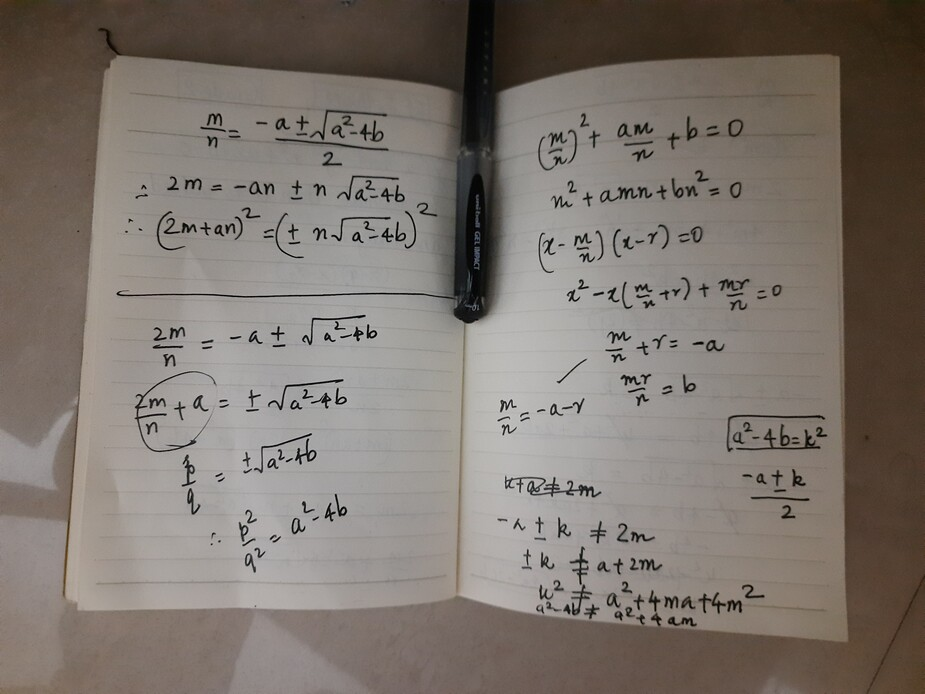
\includegraphics[scale=0.3]{struggle-1-s}
A part (and only a part because there was a long pause before he wrote the quadratic equation (\ref{eq:quadinn})--how can that pause be meaningfully captured in this ``finished text''?) of his struggle is captured herewith. Several ways were explored, many were abandoned. The author even doubted if he understands quadratic equations. Self-doubt reared its ugly head. But he persevered. 

We all enjoy reading books of history, fiction, nonfiction, etc. and finish them in a few sittings. This author has, however, learned to be at peace with spending a few slow hours without any apparent `gain' in the number of mathematical problems solved, proofs written, or pages of mathematics read. Progress in doing mathematics is slow and it is only good for our health that we accept its pace (or lack thereof). Keep calm and do math (slowly).

To be honest, however, ``keeping calm'' is only possible in the long shot or on the average (of time lived). If the author were secretly video shot during the time a satisfactory solution was not evident, a viewer (or the author himself, in retrospect) couldn't conclude that the protagonist was not agitated.
\end{reflection}
\end{enumerate}
\end{enumerate}
%%-----------------------------------------------------------------------------
\chapter{Unique Factorization}
%%%-----------------------------------------------------------------------------

%%%-----------------------------------------------------------------------------
\chapter{Linear Diophantine Equations}
%%%-----------------------------------------------------------------------------

%%%-----------------------------------------------------------------------------
\chapter{Congruences}
%%%-----------------------------------------------------------------------------

%%%-----------------------------------------------------------------------------
\appendix                                                   % Switch to appendix
%%%-----------------------------------------------------------------------------

%%%-----------------------------------------------------------------------------
\chapter{Table of Theorems}
\label{tab:theorems}
\begin{longtable}[c]{| c | c | c |}
 \caption{Theorems in the Book.}\\

 \hline
 \multicolumn{3}{| c |}{Begin List of Theorems}\\
 \hline
 Theorem & Chapter/Theorem & Notes\\
 \hline
 \endfirsthead

 \hline
 \multicolumn{3}{| c |}{Continuation of Theorems \ref{tab:theorems}}\\
 \hline
 Theorem & Chapter/Theorem & Notes\\
 \hline
 \endhead

 \hline
 \endfoot

 \hline
 \multicolumn{3}{| c |}{End List of Theorems}\\
 \hline\hline
 \endlastfoot

 Theorem [\ref{thm:gcd-multiple}] & Chapter 1 Theorem 1 & Regarding $\gcd(a/d, b/d)$.\\
 Theorem [\ref{thm:div-algo}] & Chapter 1 Theorem 2 & The Division Algorithm.\\
 Theorem [\ref{alg:euclid}] & Chapter 1 Theorem 3 & Euclid's $\gcd$ Algorithm.\\
 Theorem [\ref{thm:bezout-idty}] & Chapter 1 Theorem 4 & Bézout Identity.\\
 \end{longtable}
%%%-----------------------------------------------------------------------------

%%%-----------------------------------------------------------------------------
\MakeBibliography[nosplit]
%%%-----------------------------------------------------------------------------

%%%-----------------------------------------------------------------------------
\end{document}
%%%-----------------------------------------------------------------------------
